\documentclass[12pt]{ltjsarticle}

% 基本パッケージ
\usepackage[utf8]{inputenc}
\usepackage{luatexja}
\usepackage{amsmath, amssymb}
\usepackage{graphicx}
\usepackage{geometry}

% 表のデザインを向上させるパッケージ
\usepackage{tikz}
\usetikzlibrary{arrows.meta, positioning}
\usepackage{booktabs}
\usepackage{tabularx}
\usepackage{longtable}
\usepackage{array}
\usepackage{makecell}

% セクションやタイトルのデザイン調整
\usepackage{titlesec}
\titleformat{\section}{\normalfont\Large\bfseries}{\thesection}{1em}{}
\titleformat{\subsection}{\normalfont\large\bfseries}{\thesubsection}{1em}{}
\titleformat{\subsubsection}{\normalfont\normalsize\bfseries}{\thesubsubsection}{1em}{}

\usepackage{enumitem}
\usepackage{fontspec}

\usepackage[
  colorlinks=true,
  linkcolor=blue,
  urlcolor=cyan,
  citecolor=green
]{hyperref}

\usepackage{listing}
\usepackage{xcolor}
\newcommand{\code}[1]{\colorbox{gray!20}{\texttt{#1}}}
\usepackage{float}
\geometry{top=2cm, bottom=2cm, left=2cm, right=2cm}
\usepackage{minted}

\usemintedstyle{vs}
\setminted{
    linenos,
    frame=single,
    framesep=2mm,
    baselinestretch=1.2,
    fontsize=\small,
    breaklines
}

% 数式
\usepackage{bm}

% 画像
\usepackage{float}

\begin{document}

\title{SportEase（スポーティーズ） 学生操作説明書}
\author{行事委員会 佐藤佑作 s2301059}
\date{\today}
\maketitle
\tableofcontents

\newpage

% =====================================================================
\section{はじめに}
% =====================================================================

本書は、SportEase（スポーティーズ）の\textbf{student権限を持つ学生}向けの操作説明書である。
学生アカウントでは、大会のスコア閲覧・試合日程の確認・参加情報の確認・通知の受信など、
大会参加に必要な基本的な操作を行うことができる。

\subsection*{権限の種類}
\begin{itemize}
  \item \textbf{root} ── 最上位権限。大会設定・システム管理・ユーザー管理など全機能にアクセス可能。
  \item \textbf{admin} ── 試合進行・結果入力など大会運営補助が可能。
  \item \textbf{student} ── 本書が対象とする基本権限。マイページ・競技情報・トーナメント・通知などの参加者向け機能を利用できる。
\end{itemize}

\subsection*{クラス所属ロールについて}

初回ログイン時にクラスを選択すると、\code{クラス名\_rep} 形式のクラス所属ロールが自動的に付与される。
このロールはクラスの一員であることを示すものであり、自クラスのチーム編成管理など、追加の操作が利用できる。

学生ダッシュボードは \code{/dashboard/student/} 以下の各ページから操作する。

\subsection{学生利用時の基本方針}

学生は、大会前に自分の登録情報と競技情報を確認し、大会当日はタイムテーブル・通知・トーナメントを見ながら行動する。
表示内容は運営側の登録状況に応じて更新されるため、集合前や試合前には最新状態を確認すること。

\begin{center}
\begin{tabular}{p{4cm}p{9cm}}
\toprule
\textbf{確認タイミング} & \textbf{確認する内容} \\
\midrule
大会前 & 表示名、クラス、参加競技、競技ルール、PWAインストール状況を確認する。 \\
\midrule
登校後 & タイムテーブル、直近の試合、通知、MyID提示が必要な場所を確認する。 \\
\midrule
試合前 & 対戦相手、開始時刻、開催場所、雨天時の変更有無を確認する。 \\
\midrule
大会後 & スコア、昼競技結果、アンケート通知、過去大会アーカイブを確認する。 \\
\bottomrule
\end{tabular}
\end{center}

\subsection{大会当日の利用フロー}

以下の流れで SportEase を活用することを推奨する。
各手順の詳細は対応するセクションを参照すること。

\begin{center}
\begin{tikzpicture}[
  node distance=1.3cm,
  main/.style={
    rectangle, draw, rounded corners=4pt,
    minimum width=9cm, minimum height=0.9cm,
    text centered, fill=blue!8, font=\bfseries
  },
  opt/.style={
    rectangle, draw, dashed, rounded corners=4pt,
    minimum width=4.5cm, minimum height=0.9cm,
    text centered, fill=gray!8, font=\bfseries
  },
  arr/.style={->, thick, >=Stealth},
  optarr/.style={->, dashed, >=Stealth}
]
\node[main] (s1) {① ガイド確認・PWAインストール（事前準備）→ 第\ref{sec:guide}章};
\node[main, below of=s1] (s2) {② タイムテーブルで日程確認　→ 第\ref{sec:timetable}章};
\node[main, below of=s2] (s3) {③ トーナメント・昼競技・スコア閲覧　→ 第\ref{sec:tournament}章};
\node[main, below of=s3] (s4) {④ 通知受信・管理　→ 第\ref{sec:notification}章};

\node[opt, right=1.5cm of s2] (myid) {MyID提示（必要時）→ 第\ref{sec:myid}章};
\node[opt, right=1.5cm of s4] (req) {通知申請（任意）→ 第\ref{sec:notificationreq}章};

\draw[arr] (s1) -- (s2);
\draw[arr] (s2) -- (s3);
\draw[arr] (s3) -- (s4);
\draw[optarr] (s2.east) -- (myid.west);
\draw[optarr] (s4.east) -- (req.west);

\end{tikzpicture}
\end{center}

\subsection{初回ログイン}

\href{https://nitsche-gyouji.com}{https://nitsche-gyouji.com} をお好みのブラウザで開いてください。
すると、以下のような画面にアクセスできます。

\begin{figure}[H]
  \centering
  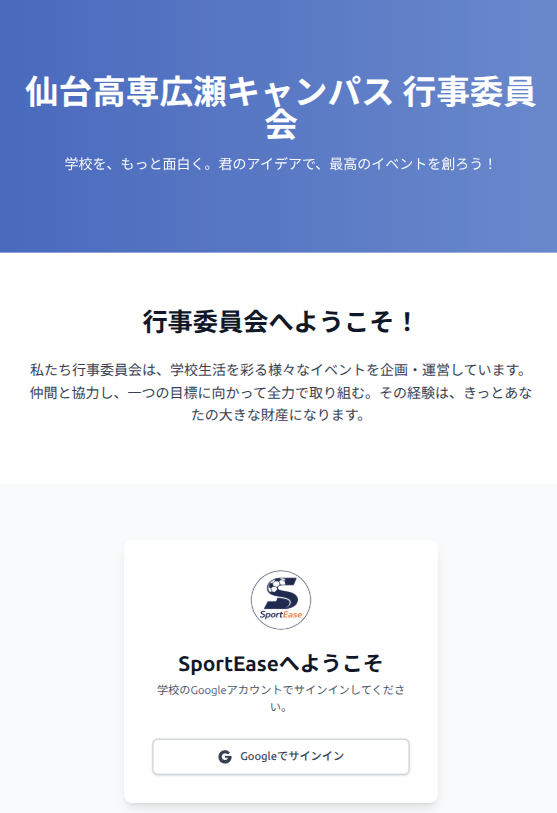
\includegraphics[width=0.8\textwidth]{./images/HP_first.png}
  \caption{アクセス結果}
\end{figure}

\texttt{Googleでサインイン}をクリックしてください。\\
\textcolor{red}{※学校のGoogle アカウントを必ず選択してください。学校のアカウント以外を選択してしまった場合は、ブラウザのキャッシュをクリアして再度アクセスしてください。}

サインインが成功すると、以下のように表示名とクラスを設定する画面に移ります。

\begin{figure}[H]
  \centering
  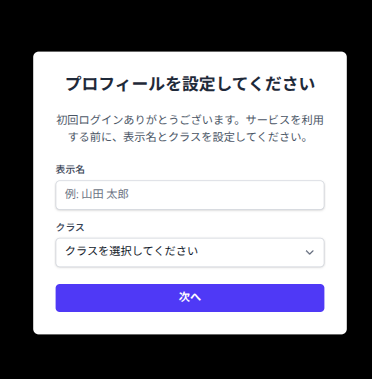
\includegraphics[width=0.8\textwidth]{./images/set-display-name.png}
  \caption{表示名とクラス設定画面}
\end{figure}

ここで、アプリ内での表示名とクラスを決定してください。
確認画面も表示されるので、クラスに関しては間違えないようにお願いします。

\newpage

% =====================================================================
\section{マイページ}
% =====================================================================

\textbf{ページ}: \code{/dashboard/student/my-page}

自分のクラスに関する情報を一覧で確認できるページである。

\begin{figure}[H]
  \centering
  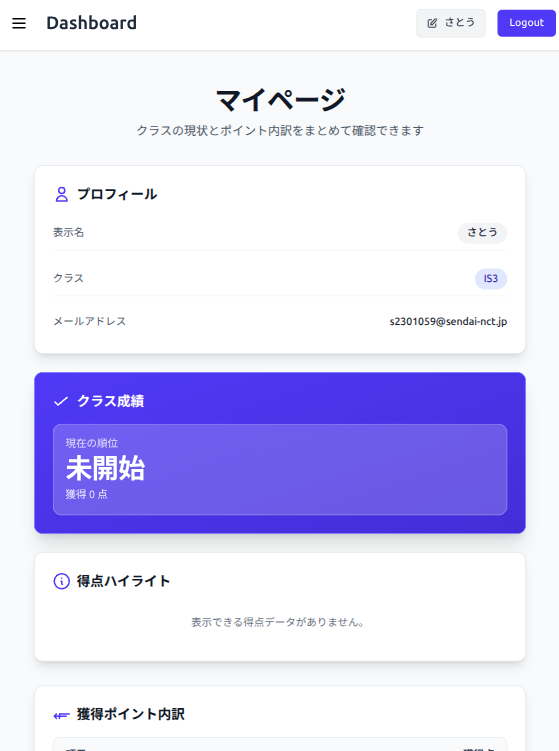
\includegraphics[width=0.8\textwidth]{./images/student-mypage.png}
  \caption{マイページ画面}
\end{figure}

\subsection{クラスのスコアと順位}

現在の大会におけるクラスの合計得点と順位を表示する。
得点の内訳（競技別・カテゴリ別）も確認できる。
rootの設定によりスコアが非表示になっている場合は、順位や得点が表示されないことがある。

\subsection{直近の試合スケジュール}

自クラスが出場する直近の試合の日時・場所・対戦相手を確認できる。
集合前にこの欄を確認し、試合開始時刻に遅れないように移動する。

\subsection{アンケートへのアクセス}

大会終了後にrootからアンケートが配信された場合、マイページからアンケートURLへアクセスできる。

\subsection{クラスの試合進捗}

自クラスの全競技にわたるトーナメント進捗状況を確認できる。

\newpage

% =====================================================================
\section{トーナメント情報}\label{sec:tournament}
% =====================================================================

\textbf{ページ}: \code{/dashboard/student/tournament}

大会の全競技にわたるトーナメントブラケットを確認するページである。

\begin{figure}[H]
  \centering
  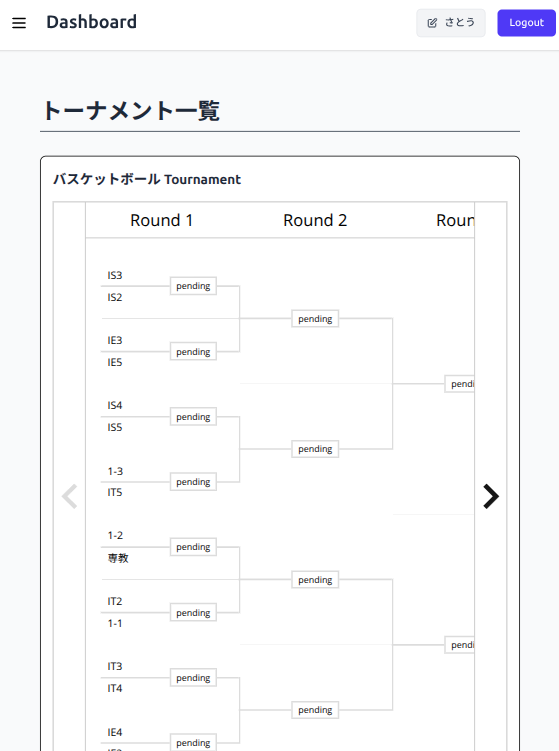
\includegraphics[width=0.8\textwidth]{./images/student-tournament-list.png}
  \caption{トーナメント画面}
\end{figure}

\subsection{トーナメントブラケットの閲覧}

競技ごとのトーナメント対戦表を表示する。
各試合の対戦クラス・日時・結果を確認できる。
自クラスの試合だけでなく、次に対戦する可能性があるクラスも確認できる。
試合結果が入力されると、勝ち上がり先の表示も更新される。

\subsection{雨天時のブラケット}

雨天時モードが有効な場合、雨天時に対応したブラケット（敗者復活戦追加後）も表示される。
雨天時モードでは、グラウンド競技や昼競技の扱いが変更される場合がある。
当日の案内と画面表示を合わせて確認する。

\newpage

% =====================================================================
\section{タイムテーブル}\label{sec:timetable}
% =====================================================================

\textbf{ページ}: \code{/dashboard/student/timetable}

大会全体の試合スケジュールを時系列で確認するページである。

\begin{figure}[H]
  \centering
  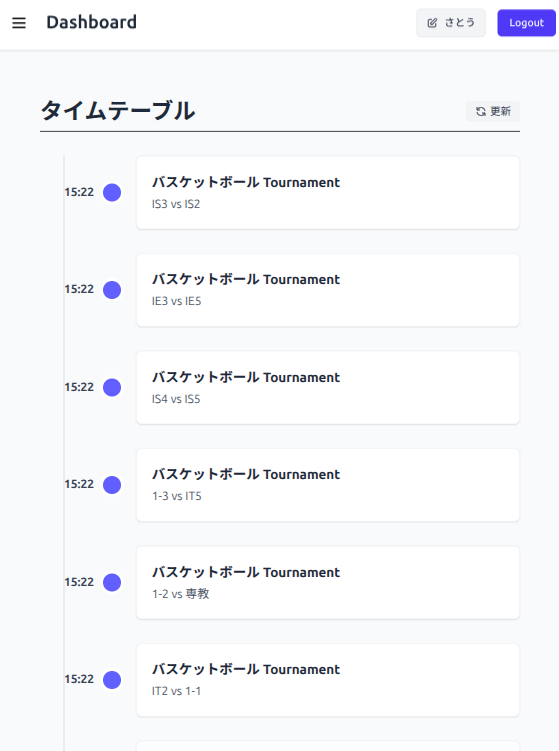
\includegraphics[width=0.8\textwidth]{./images/student-timetable.png}
  \caption{タイムテーブル画面}
\end{figure}

\subsection{試合一覧の確認}

全競技の試合日時・開催場所・対戦クラスを一覧で表示する。
通常時および雨天時の開始時間を確認できる。
自分のクラスだけでなく、他クラスや他競技の進行状況も確認できる。
開始時間が変更された場合は、運営からの通知と合わせて最新情報を確認する。

\subsection{昼競技のスケジュール}

トーナメント競技に加えて、昼競技（Noon Game）の日程も表示される。
昼休みに移動が必要な場合は、午前中のうちに集合場所と開始時刻を確認しておく。

\newpage

% =====================================================================
\section{昼競技（Noon Game）情報}
% =====================================================================

\textbf{ページ}: \code{/dashboard/student/noon-game}

昼休みに行われる特別競技（昼競技）の詳細を確認するページである。

\begin{figure}[H]
  \centering
  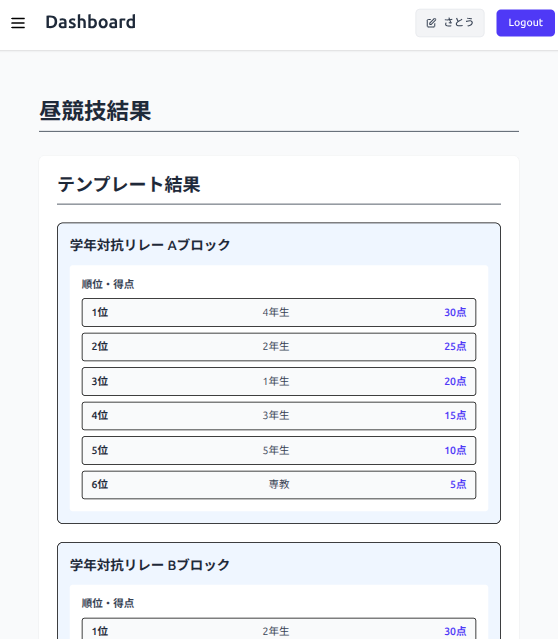
\includegraphics[width=0.8\textwidth]{./images/student-noon-game-result.png}
  \caption{昼競技結果}
\end{figure}

\subsection{セッション情報の確認}

現在の昼競技セッションの概要・ポイント設定を確認できる。
勝利点、引き分け点、参加点など、通常競技とは異なる点数ルールが設定される場合がある。

\subsection{試合結果の確認}

各試合（年リレー・コースリレー・綱引きなど）の進行状況と結果を閲覧できる。

\subsection{クラス別ポイントの確認}

昼競技で各クラスが獲得したポイントの集計を確認できる。
結果入力直後は集計が更新されるため、表示が古い場合は再読み込みして確認する。

\newpage

% =====================================================================
\section{競技情報}
% =====================================================================

\textbf{ページ}: \code{/dashboard/student/sport-info}

大会で実施される各競技の詳細情報を確認するページである。

\begin{figure}[H]
  \centering
  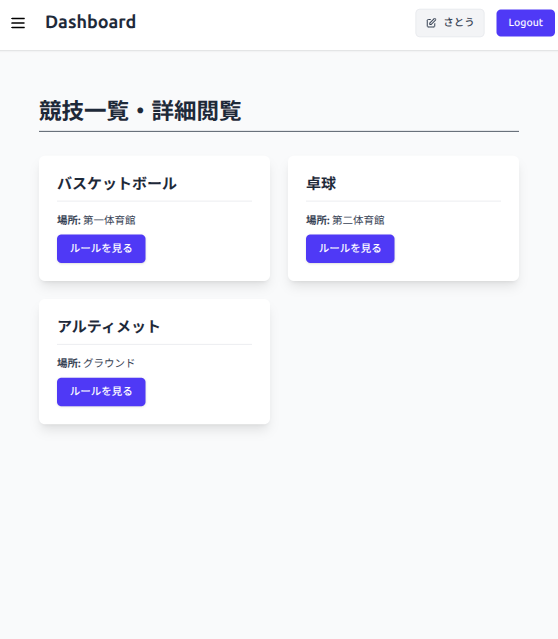
\includegraphics[width=0.8\textwidth]{./images/student-sports-info.png}
  \caption{競技情報閲覧画面}
\end{figure}

\subsection{競技一覧の閲覧}

大会に登録されている全競技の名称・開催場所・概要を一覧で確認できる。
自分が参加しない競技でも、応援や移動のために開催場所を確認できる。

\subsection{ルールの確認}

各競技のルールPDFを閲覧できる。
競技ごとの集合場所、持ち物、禁止事項が記載されている場合があるため、試合前に確認する。

\newpage

% =====================================================================
\section{スコア一覧}
% =====================================================================

\textbf{ページ}: \code{/dashboard/student/score-list}

全クラスの得点状況を確認するページである。
なお、rootの設定によってスコアが非表示になる場合がある。

\begin{figure}[H]
  \centering
  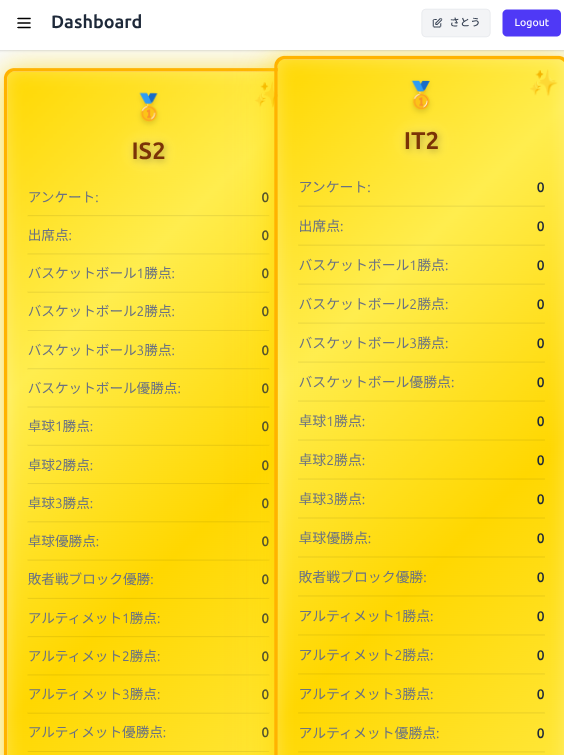
\includegraphics[width=0.8\textwidth]{./images/student-score.png}
  \caption{スコア一覧画面}
\end{figure}

\subsection{クラス別スコアの閲覧}

全クラスの合計得点とランキングを確認できる。

\subsection{得点内訳の確認}

クラスごとの得点は以下のカテゴリ別に内訳が表示される。

\begin{itemize}
  \item \textbf{初期ポイント} ── 大会開始時の基礎点
  \item \textbf{アンケートポイント} ── アンケート参加による加点
  \item \textbf{出席ポイント} ── 出席状況に応じた加点
  \item \textbf{トーナメント順位} ── 1位・2位・3位・優勝による獲得ポイント
  \item \textbf{昼競技ポイント} ── 昼競技の結果による加点
\end{itemize}

スコアは運営の結果入力や出席登録に応じて更新される。
表示内容に疑問がある場合は、運営スタッフに確認する。

\newpage

% =====================================================================
\section{MyIDによる参加確認}\label{sec:myid}
% =====================================================================

MyIDによる参加確認では、学生側でバーコードを発行する操作は不要である。
大会当日に運営スタッフから案内があった場合は、学生証等のMyIDバーコードを提示する。

運営スタッフはMyIDバーコードを読み取り、対象競技への参加本登録とラウンドチェックインを行う。
MyIDバーコードは \code{H10} に7桁の学籍番号が続く形式（例: \code{H102301059}）として扱われる。

\subsection{当日の流れ}

\begin{enumerate}
  \item 事前に自分が参加する競技へエントリーされていることを確認する。
  \item 受付または競技開始前の案内に従い、運営スタッフへMyIDバーコードを提示する。
  \item 読み取りが完了すると、参加本登録および対象ラウンドへのチェックインが行われる。
\end{enumerate}

\subsection{注意事項}

MyIDバーコードが読み取れない場合は、運営スタッフに学籍番号を伝えて手入力で確認してもらう。
ただし、対象競技に事前エントリーされていない場合は参加本登録できない。
学生側でSportEase上にバーコードを表示する操作はない。
学生証等、MyIDを確認できるものを忘れないようにする。


\newpage

% =====================================================================
\section{通知}\label{sec:notification}
% =====================================================================

\textbf{ページ}: \code{/dashboard/student/notification}

運営から配信された通知を受信・管理するページである。

\begin{figure}[H]
  \centering
  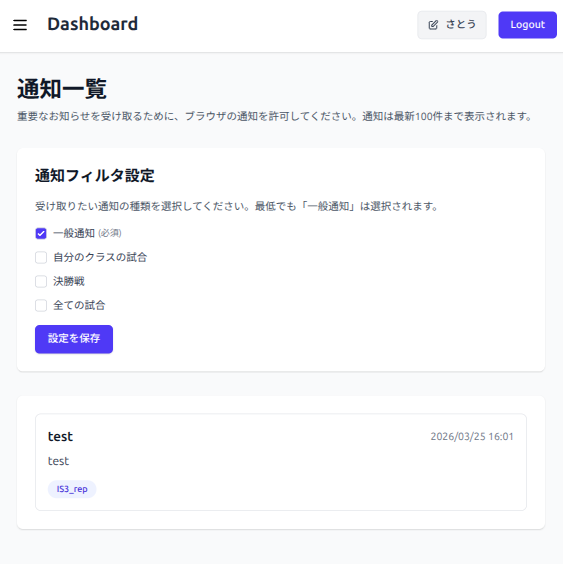
\includegraphics[width=0.8\textwidth]{./images/student-receive-notice.png}
  \caption{通知画面}
\end{figure}

\subsection{通知の確認}

受信した通知の一覧を表示する。最新100件まで確認できる。
重要な連絡は通知一覧に残るため、Push通知を見逃した場合でもこの画面から確認できる。

\subsection{通知のフィルタリング}

以下の通知タイプごとに表示・非表示を切り替えられる。

\begin{itemize}
  \item \textbf{一般通知} ── 運営からの全体向けお知らせ（常に表示）
  \item \textbf{自分のクラスの試合} ── 自クラスが出場する試合の通知
  \item \textbf{決勝戦} ── 決勝戦に関する通知
  \item \textbf{全試合} ── 全試合に関する通知
\end{itemize}

一般通知は必須であり、常に受信対象となる。
試合関連の通知を多く受け取りたい場合は「全試合」を有効にし、自分のクラスに関係する通知だけでよい場合は
「自分のクラスの試合」を有効にする。

\subsection{プッシュ通知の設定}

ブラウザのプッシュ通知を有効にすることで、ページを開いていない状態でも通知を受け取ることができる。
プッシュ通知の登録・解除はダッシュボードから行う。
通知が届かない場合は、ブラウザの通知許可、OS側の通知設定、PWAとしてインストール済みかを確認する。
iOSでは、ホーム画面に追加したPWAから開いた場合のみPush通知が有効になることがある。

\begin{figure}[H]
  \centering
  \includegraphics[width=0.8\textwidth]{./dashboard-notice-setting.png}
  \caption{プッシュ通知の有効化}
\end{figure}

\newpage

% =====================================================================
\section{通知申請}\label{sec:notificationreq}
% =====================================================================

\textbf{ページ}: \code{/dashboard/student/notification-request}

運営に対して通知の配信を申請するページである。
申請はroot権限の担当者が審査し、承認された場合に通知が配信される。

\begin{figure}[H]
  \centering
  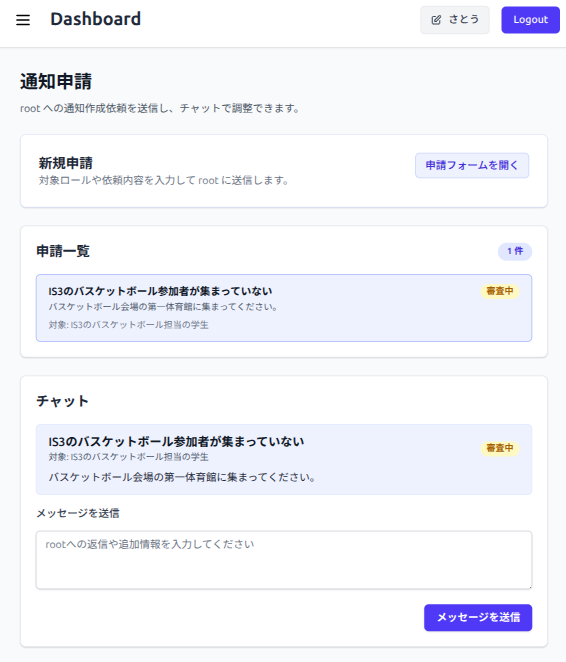
\includegraphics[width=0.8\textwidth]{./images/student-notice-req.png}
  \caption{通知申請画面}
\end{figure}

\subsection{申請の作成}

通知のタイトル・本文・対象情報を入力して申請を提出する。
申請内容はrootが確認するため、配信したい理由、対象者、希望する配信タイミングを本文に含める。
緊急性が高い場合は、申請だけでなく近くの運営スタッフにも直接伝える。

\subsection{申請状況の確認}

提出済みの申請一覧と、各申請の審査状況を確認できる。
審査状況は以下のいずれかで表示される。

\begin{center}
\begin{tabular}{lp{9cm}}
\toprule
\textbf{ステータス} & \textbf{説明} \\
\midrule
審査中 & 申請が提出され、rootによる審査を待っている状態。 \\
承認済み & 申請が承認され、通知が配信された状態。 \\
否認 & 申請が否認された状態。 \\
\bottomrule
\end{tabular}
\end{center}

rootから追加確認のメッセージが届く場合がある。
申請後は審査状況とメッセージ欄を確認し、必要に応じて返信する。

\newpage

% =====================================================================
\section{過去大会のアーカイブ}
% =====================================================================

\textbf{ページ}: \code{/dashboard/archive}

過去に開催された大会の記録を閲覧するページである。

\subsection{大会の検索}

年度・シーズン（春季・秋季）で過去の大会を絞り込んで参照できる。
現在の大会が終了してアーカイブされると、過去大会として参照できるようになる。

\subsection{過去大会の結果確認}

選択した大会のクラス別スコアやランキングを確認できる。
大会後の振り返りや次回大会の参考として利用できる。

\newpage

% =====================================================================
\section{ガイド}\label{sec:guide}
% =====================================================================

\textbf{ページ}: \code{/dashboard/guide}

アプリの利用に関する各種案内を確認するページである。

\begin{figure}[H]
  \centering
  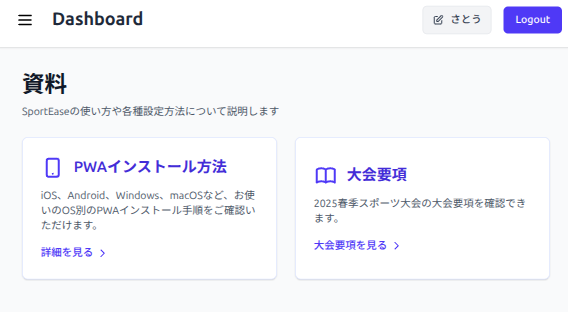
\includegraphics[width=0.8\textwidth]{./images/student-guide.png}
  \caption{ガイド画面}
\end{figure}

\subsection{PWAインストール手順}

SportEaseをスマートフォンのホーム画面に追加する手順を確認できる。
iOS・Androidそれぞれの操作手順が掲載されている。
大会当日は通知やタイムテーブルをすぐ確認できるため、事前にPWAとして追加しておくことを推奨する。

\subsection{競技要項PDFの閲覧}

rootがアップロードした競技要項PDFをここから参照できる。
大会要項のほか、rootが追加した会場図や補足資料などのPDFも表示される場合がある。
資料が更新された場合は、同じページから最新のPDFを開くことができる。


\newpage

% =====================================================================
\section{クラス情報}
% =====================================================================

\textbf{ページ}: \code{/dashboard/student/class-info}

\code{クラス名\_rep} ロールを持つ学生がアクセスできるページである。

\begin{figure}[H]
  \centering
  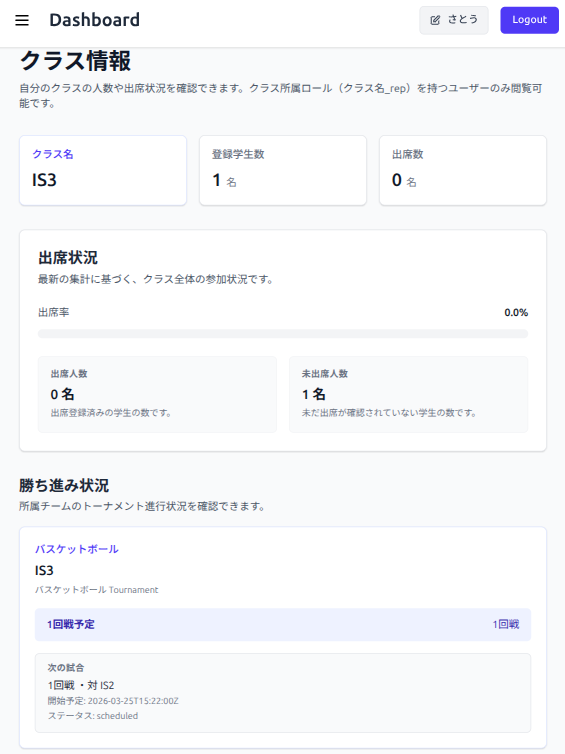
\includegraphics[width=0.8\textwidth]{./images/student-class-info.png}
  \caption{クラス情報画面}
\end{figure}

\subsection{クラスの概要確認}

クラス名・登録学生数・出席者数・出席率を確認できる。

\subsection{メンバー一覧の確認}

クラス内の全メンバーの競技別チーム割り当て状況を一覧で確認できる。
自分やクラスメンバーの参加競技が正しく登録されているか確認する。

\subsection{試合進捗の確認}

自クラスの全競技にわたるトーナメント進捗状況を確認できる。
学生はこの画面を使って、次の試合予定や未確認の競技を把握できる。

\newpage

% =====================================================================
\section{機能一覧まとめ}
% =====================================================================

以下にstudent権限で利用可能な操作を一覧にまとめる。

\begin{longtable}{p{4.5cm}p{9cm}}
\toprule
\textbf{機能} & \textbf{概要} \\
\midrule
\endhead
マイページの閲覧 & クラスのスコア・順位・直近の試合スケジュールを確認 \\
\midrule
トーナメントの閲覧 & 競技ごとのトーナメントブラケットと試合結果を確認 \\
\midrule
タイムテーブルの閲覧 & 全競技の試合日時・場所・対戦クラスを一覧で確認 \\
\midrule
昼競技情報の閲覧 & 昼競技のセッション情報・試合結果・ポイントを確認 \\
\midrule
競技情報の閲覧 & 各競技のルール・開催場所・概要を確認 \\
\midrule
スコア一覧の閲覧 & 全クラスの得点・ランキング・カテゴリ別内訳を確認 \\
\midrule
MyIDによる参加確認 & 大会当日にMyIDバーコードを提示し、運営スタッフによる参加本登録を受ける \\
\midrule
通知の受信・フィルタリング & 運営からの通知を受信し、種別ごとに表示を管理 \\
\midrule
プッシュ通知の設定 & ブラウザのプッシュ通知を登録・解除 \\
\midrule
通知申請の提出 & 運営への通知配信申請を作成・提出 \\
\midrule
申請状況の確認 & 提出済み申請の審査状況とメッセージを確認 \\
\midrule
過去大会の閲覧 & アーカイブから過去大会のスコアや結果を参照 \\
\midrule
ガイドの閲覧 & PWAインストール手順・競技要項PDFを確認 \\
\midrule
クラス情報の閲覧 & クラスの出席状況・メンバー一覧・試合進捗を確認 \\
\bottomrule
\end{longtable}

\end{document}
